  \begin{figure}
    \centering

    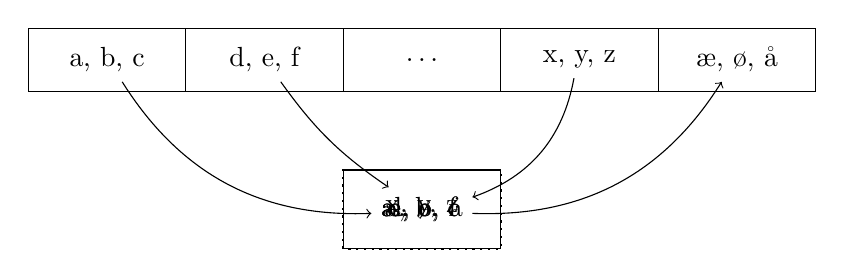
\begin{tikzpicture}
      % Block 1
      \draw[] (0,0)  rectangle ++(2,0.8) node[pos=.5] (b1) {a, b, c};

      % Block 2
      \draw[] (2,0)  rectangle ++(2,0.8) node[pos=.5] (b2) {d, e, f};

      % Block 3
      \draw[] (4,0)  rectangle ++(2,0.8) node[pos=.5] {$\dots$};

      % Block 4
      \draw[] (6,0)  rectangle ++(2,0.8) node[pos=.5] (b3) {x, y, z};

      % Block 5
      \onslide<10-> {
        \draw[] (8,0) rectangle ++(2,0.8) node[pos=.5] (b4) {\ae, \o, \aa};
      }

      % Memory
      \draw[dotted, thick] (4,-2) rectangle ++(2,1) node[pos=.5] (M) {};

      % NOTE: Tikz does not like \only<>/\onslide<> within a node's text (even
      % if the output seems correct. So to not get compiler errors it must be
      % copy-pasted...
      %
      % On the bright side, it also gives a very cool "active block" effect.
      \onslide<2> {
        \draw[] (4,-2) rectangle ++(2,1) node[pos=.5] (M) {a, b, c};
      }
      \onslide<3> {
        \draw[] (4,-2) rectangle ++(2,1) node[pos=.5] (M) {d, e, f};
      }
      \onslide<5> {
        \draw[] (4,-2) rectangle ++(2,1) node[pos=.5] (M) {x, y, z};
      }
      \onslide<7> {
        \draw[] (4,-2) rectangle ++(2,1) node[pos=.5] (M) {\ae\phantom{, \o, \aa}};
      }
      \onslide<8> {
        \draw[] (4,-2) rectangle ++(2,1) node[pos=.5] (M) {\ae, \o\phantom{, \aa}};
      }
      \onslide<9> {
        \draw[] (4,-2) rectangle ++(2,1) node[pos=.5] (M) {\ae, \o, \aa};
      }

      % Arrows
      \onslide<2>  { \draw[->] (b1) edge[bend right]    (M); }
      \onslide<3>  { \draw[->] (b2) edge[bend right=10] (M); }
      \onslide<5>  { \draw[->] (b3) edge[bend left]     (M); }
      \onslide<10> { \draw[->] (M)  edge[bend right]    (b4); }
    \end{tikzpicture}
  \end{figure}
